\documentclass{beamer}

\usepackage{listings}
\usepackage{xcolor}

% Define custom colors
\definecolor{mygreen}{rgb}{0,0.6,0}
\definecolor{mygray}{rgb}{0.5,0.5,0.5}
\definecolor{myblue}{rgb}{0.1,0.1,0.8}
\definecolor{myred}{rgb}{0.8,0.1,0.1}

% Configure listings
\lstset{
  language=C++,
  basicstyle=\ttfamily\tiny,    % Small font size
  keywordstyle=\color{myblue},   % Keywords in blue
  commentstyle=\color{mygreen},  % Comments in green
  stringstyle=\color{myred},     % Strings in red
  numberstyle=\tiny\color{mygray}, % Line numbers in gray
  numbers=left,                  % Line numbers on the left
  stepnumber=1,                  % Line number step
  numbersep=5pt,                 % Space between line numbers and code
  backgroundcolor=\color{white}, % Background color of the code
  showspaces=false,              % Do not show spaces
  showstringspaces=false,        % Do not show spaces in strings
  showtabs=false,                % Do not show tabs
  frame=single,                  % Single frame around code
  tabsize=2,                     % Tab size
  captionpos=b,                  % Caption position
  breaklines=true,               % Automatic line breaking
  breakatwhitespace=true,        % Line breaks at whitespaces
  title=\lstname,                % Show filename as title
}

\usetheme{Madrid}

\title{Prezentare Proiect SC}
\author{David P. Dudas}
\date{2024}

\begin{document}

\begin{frame}
  \titlepage
\end{frame}

\begin{frame}{Cuprins}
  \tableofcontents
\end{frame}

\section{DES}

\begin{frame}{DES (Data Encryption Standard)}
  \begin{itemize}
    \item Algoritm de criptare simetrică cu cheie de 56 biți
    \item Utilizat în mod extensiv în anii 1970 și 1980
    \item Structură: 16 runde de permutări și substituții
    \item Dimensiunea blocului criptat: 64 biți
  \end{itemize}
\end{frame}

\begin{frame}{DES Diagram}
  \begin{figure}
    \centering
    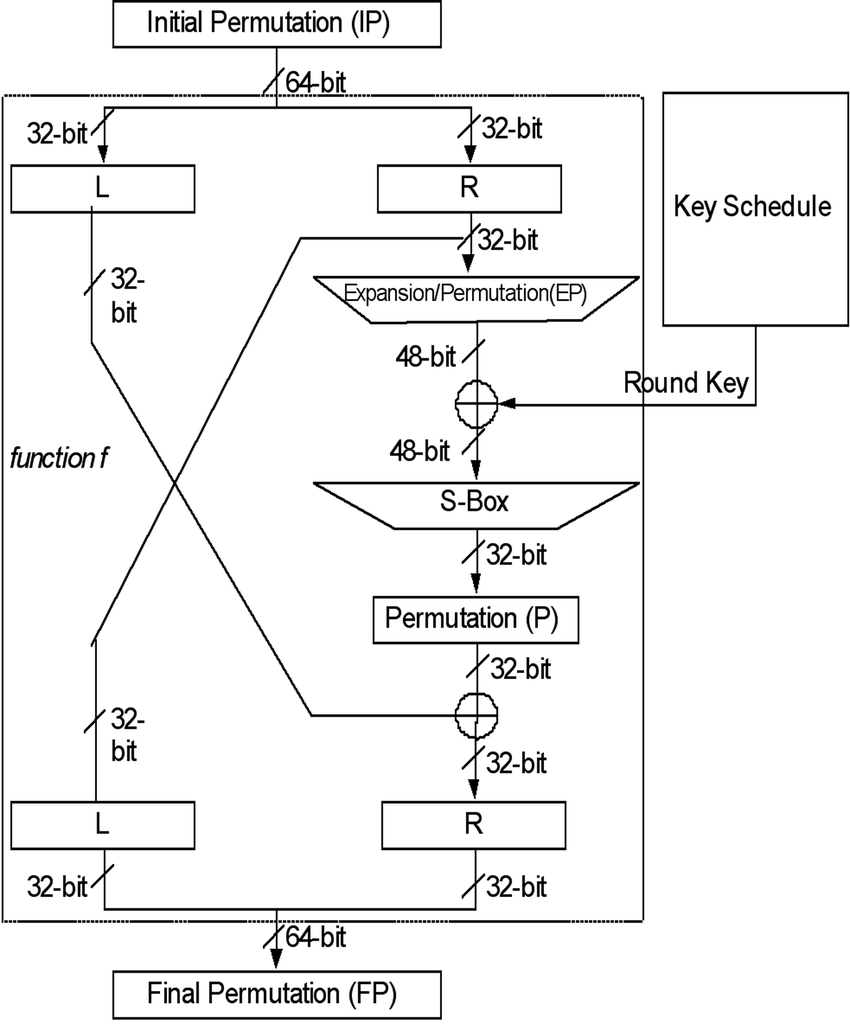
\includegraphics[width=0.5\textwidth]{images/des_diagram.png}
  \end{figure}
\end{frame}

\begin{frame}[fragile]{Implementare DES în C++}
  \begin{block}{Header-ul clasei DES}
    \begin{lstlisting}[language=C++]
class DES : public ICryptographicAlgorithm
{
public:
  void encrypt(IOConfig& ioConfig) override;
  void decrypt(IOConfig& ioConfig) override;
private:
  const std::vector<std::bitset<48>> generateKeys(const std::bitset<64>& key);
  const std::bitset<64> keyStringToBitset(std::string& keyStr);
  const std::bitset<64> applyPermutations(std::bitset<64>& block, std::vector<std::bitset<48>>& subKeys);
  const void applyPermutationsOnChunks(IOConfig& ioConfig, std::vector<std::bitset<48>>& subKeys);
  const std::bitset<64> convertCharBufferToBitset(const char* buffer, int bufferSize);
  const void addPaddingToBitset(std::bitset<64>& block, int originalSize);
  const std::bitset<56> initialKeyPermutation(const std::bitset<64>& key);
  const std::bitset<28> leftCircularShift(std::bitset<28>& halfKey, int shifts);
  const std::bitset<64> applyInitialPermutation(const std::bitset<64>& block);
  const std::bitset<32> feistelFunction(const std::bitset<32>& halfBlock, const std::bitset<48>& key);
  const void applyFeistelFunction(std::bitset<64>& permutedBlock, std::vector<std::bitset<48>>& subKeys);
  const std::bitset<48> createExpandedBlock(const std::bitset<32>& halfBlock);
  const std::bitset<32> applySubstitutionBoxesPermutations(const std::bitset<48>& xored);
  const std::bitset<32> applyFinalPermutation(const std::bitset<32>& block);
  const std::bitset<64> applyInversePermutation(const std::bitset<64>& permutedBlock);
};
    \end{lstlisting}
  \end{block}
\end{frame}

\section{AES}

\begin{frame}{AES (Advanced Encryption Standard)}
  \begin{itemize}
    \item Algoritm de criptare simetrică cu chei de 128, 192, sau 256 biți
    \item Aprobat ca standard de criptare în 2001
    \item Structură: 10, 12, sau 14 runde de substituții, permutări și mixări
    \item Dimensiunea blocului criptat: 128 biți
  \end{itemize}
\end{frame}

\begin{frame}{AES Diagram}
  \begin{figure}
    \centering
    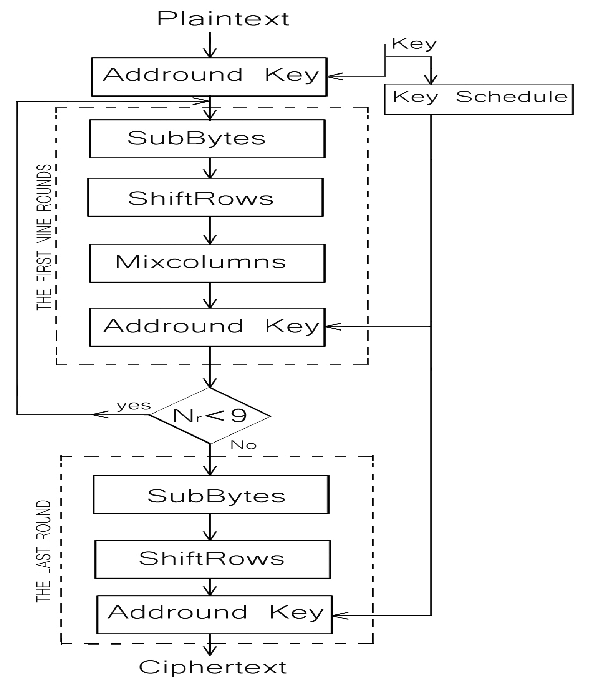
\includegraphics[width=0.5\textwidth]{images/aes_diagram.png}
  \end{figure}
\end{frame}

\begin{frame}[fragile]{Implementare AES în C++}
  \begin{block}{Header-ul clasei AES}
    \begin{lstlisting}[language=C++]
class AES : public ICryptographicAlgorithm
{
  u_int8_t numberOfRounds;
  u_int8_t keyCoefficient;
  static const u_int8_t blockSize = 16;
  void keyExpansionCore(std::bitset<8> word[4], int rconIterationCount);
  std::vector<std::bitset<8>> keyExpansion(const std::string& key);
  void addPKCS7Padding(std::vector<std::bitset<8>>& block);
  void removePKCS7Padding(std::vector<std::bitset<8>>& data);
  std::vector<std::bitset<8>> convertCharBufferToBitsetVector(const char* buffer, size_t length);
  void encryptBlock(std::vector<std::bitset<8>>& plaintext, const std::vector<std::bitset<8>>& expandedKeys);
  void subBytes(std::vector<std::bitset<8>>& state);
  void shiftRows(std::vector<std::bitset<8>>& state);
  void mixColumns(std::vector<std::bitset<8>>& state);
  void decryptBlock(std::vector<std::bitset<8>>& ciphertext, const std::vector<std::bitset<8>>& expandedKeys);
  void invSubBytes(std::vector<std::bitset<8>>& state);
  void invShiftRows(std::vector<std::bitset<8>>& state);
  void invMixColumns(std::vector<std::bitset<8>>& state);
  void addRoundKey(std::vector<std::bitset<8>>& state, const std::vector<std::bitset<8>>& roundKey);
public:
    AES(Algorithms algorithm);
    void encrypt(IOConfig& ioConfig) override;
    void decrypt(IOConfig& ioConfig) override;
};
    \end{lstlisting}
  \end{block}
\end{frame}

\section{RSA}

\begin{frame}{RSA (Rivest-Shamir-Adleman)}
  \begin{itemize}
    \item Algoritm de criptare asimetrică cu două chei: publică și privată
    \item Bazat pe factorizarea numerelor mari
    \item Utilizat pentru securizarea transmisiilor de date
    \item Dimensiunea blocului criptat: variabilă, în funcție de lungimea cheii utilizate
  \end{itemize}
\end{frame}

\begin{frame}{RSA Algorithm}
  \begin{itemize}
    \item \textbf{Generare de cheie:}
    \begin{itemize}
      \item Se aleg două numere prime mari $p$ și $q$
      \item Se calculează $n = p \times q$
      \item Se calculează $\phi(n) = (p-1) \times (q-1)$
      \item Se alege un număr $e$ astfel încât $1 < e < \phi(n)$ și $cmmmc(e, \phi(n)) = 1$
      \item Se calculează inversul multiplicativ modular $d$ al lui $e$ modulo $\phi(n)$
      \item Cheia publică: $(e, n)$
      \item Cheia privată: $(d, n)$
    \end{itemize}
    \item \textbf{Criptare:}
    \begin{itemize}
      \item Dând un mesaj în clar $m$, se calculează mesajul criptat $c$ folosind formula $c = m^e \mod n$
    \end{itemize}
    \item \textbf{Decriptare:}
    \begin{itemize}
      \item Dând un mesaj criptat $c$, se calculează mesajul în clar $m$ folosind formula $m = c^d \mod n$
    \end{itemize}
  \end{itemize}
\end{frame}

\begin{frame}[fragile]{Implementare RSA în C++}
  \begin{block}{Header-ul clasei RSA}
    \begin{lstlisting}[language=C++]
class RSA : public ICryptographicAlgorithm
{
public:
  void generateKeys(IOConfig& ioConfig);
  void encrypt(IOConfig& ioConfig) override;
  void decrypt(IOConfig& ioConfig) override;
private:
  void saveKey(const std::string& filename, const mpz_class& a, const mpz_class& b);
  void loadKey(const std ::string& filename, mpz_class& a, mpz_class& b);
  mpz_class generateLargePrime();
  mpz_class rsaEncrypt(const mpz_class& m, const mpz_class& e, const mpz_class& n);
  mpz_class rsaDecrypt(const mpz_class& c, const mpz_class& d, const mpz_class& n);
  const int keyBitSize = 1024;
};
    \end{lstlisting}
  \end{block}
\end{frame}

\section{Concluzii}

\begin{frame}{Concluzii}
  \begin{itemize}
    \item Utilizarea bibliotecii GMP pentru operații cu numere mari a ușurat implementarea RSA
    \item Testarea algoritmilor pe fișiere de dimensiuni diferite a fost realizată
  \end{itemize}
\end{frame}

\begin{frame}[plain]
  \centering
  \Huge\bfseries
  \textcolor{myblue}{Sfârșit}
\end{frame}

\end{document}
